\documentclass[a4paper,10pt]{article}

\usepackage{graphicx}
\usepackage{graphicx}
\usepackage{color}
\usepackage{amsbsy}
\usepackage{mathrsfs}
\usepackage{mathpazo,bm}
\usepackage{amsmath}
\usepackage{multirow}


\newcommand{\pencil}{{\sc Pencil}}
\newcommand{\pencilcode}{{\sc Pencil Code}}
\newcommand{\pderiv}[2]{\frac{\partial #1}{\partial #2}}
\newcommand{\pderivn}[3]{\frac{{\partial{}}^{#3} #1}{{\partial #2}^{#3}}}
%\newcommand{\aderiv}[1]{\frac{{\mathcal D} #1}{{\mathcal D}t}}
\newcommand{\aderiv}[1]{\frac{D #1}{Dt}}
\newcommand{\ee}{\mathrm{e}}
\newcommand{\ttimes}[1]{10^{#1}}
\newcommand{\xtimes}[2]{#1 \times 10^{#2}}
\newcommand{\xstimes}[3]{(#1 \pm #2) \times 10^{#3}}
\newcommand{\vt}[1]{\mathbf{#1}}       %for tensors
\renewcommand{\v}[1]{{\boldsymbol #1}} %for vectors

\newcommand{\del}{\v{\nabla}}
\newcommand{\grad}{\del}
\newcommand{\Div}{\v{\nabla}\cdot}
\newcommand{\curl}{\v\nabla\times}
\newcommand{\Laplace}{\nabla^2}
\newcommand{\de}{\mathrm{d}} 
\newcommand{\rint}{$s_{\rm int}\,$}
\newcommand{\rext}{$s_{\rm ext}\,$}
\newcommand{\hatr}{\hat{\v{r}}}
\newcommand{\hats}{\hat{\v{s}}}
\newcommand{\hatphi}{\hat{\v{\phi}}}
\newcommand{\hatz}{\hat{\v{z}}}
\newcommand{\va}{v_{_{\rm A}}}
\newcommand{\degree}{\ensuremath{^\circ}}

\begin{document}
\date{}


\title{{\bf ``Hello, disk!'' with the \pencilcode}}


\author{Wlad Lyra\\
{\it Uppsala University}}               
\date{}  

\maketitle


\section{Introduction}

This file is intended to be a guide on how to setup a simulation using the \pencilcode. It will tour through the configuration files, then through the start and finally run parameters. We choose a simple 2D problem that is conceptually simple and can at the same time, highlight some of the nuances of the code better than a 1D problem. The problem we choose is to set up a differentially rotating accretion disk around a central star of mass $M$. We make the approximations of isothermality, laminarity (as opposed to turbulence), and axis-symmetry, as well as ignoring the disk's self-gravity. Shock terms are also ignored. 

The equations to solve are the continuity and Navier-Stokes equations in an inertial frame

\begin{equation}
\label{continuity}
  \aderiv{\rho} = -\rho{\Div\v{u}}, 
\end{equation}

\begin{equation}
\label{navierstokes}
  \aderiv{\v{u}} = -\frac{1}{\rho}\grad{p} - \frac{GM}{r^3}\v{r} + \nu\Laplace{\v{u}}
\end{equation}where $\rho$ and $\v{u}$ are the density and velocity of the gas, $p$ is the pressure, $G$ is the gravitational constant and $\nu$ is the kinematic viscosity. The operator ${D}/Dt = \partial /{\partial}t + \v{u}\cdot\del$ represents the advective derivative.

We write cylindrical coordinates as ($s$,$\phi$,$z$) and spherical coordinates as ($r$,$\phi$,$\theta$), where $\theta$ is the polar angle and $\phi$ the azimuthal angle. The $z$ direction is perpendicular to the midplane of the disk.

The Navier-Stokes equation are in fact three equations, one for each component of the velocity field. In cylindrical coordinates and under the conditions of azimuthal symmetry ($\partial /{\partial}\phi$=0) and initial centrifugal balance $u_{r}(t_0)$=0, they read

\begin{eqnarray}
\ddot{s} - s{\dot{\phi}}^2 &=&  -\frac{1}{\rho}\pderiv{p}{s} - \frac{GM}{r^3}s\\ 
s\ddot{\phi}  &=&  \nu \left(\pderivn{s\dot\phi}{s}{2} + \frac{1}{s}\pderiv{s\dot{\phi}}{r} - \frac{\dot\phi}{s} \right)\\
\ddot{z}  &=& -\frac{1}{\rho}\pderiv{p}{z} - \frac{GM}{r^3}z 
\end{eqnarray}

The first equation gives the condition for initial centrifugal balance ($\ddot{s}$=0)

\begin{equation}
  \label{centrifugal}
  \Omega^2 = \Omega_{\rm K}^2 + \frac{1}{s\rho}\pderiv{p}{s} 
\end{equation}where we substituted $\Omega_{\rm K}=GM/r^3$ for the Keplerian angular frequency and $\Omega=\dot\phi$ for the true (pressure-corrected) angular frequency.

The second one explicits that viscosity is continuously depriving the disk of angular momentum and making it acreete into the central star. Although, as $\nu$ is small, this effect takes many orbits to settle into a steady inflow. 

The third equation gives the condition for hydrostatic equilibrium ($\ddot{z}$=0)

\begin{equation}
  \frac{1}{\rho}\pderiv{p}{z} = -\Omega_{\rm K} z 
\end{equation}

This last equation will be ignored in this problem, but we state it for the sake of completeness. 

Our job is to code this initial condition.

\section{Initial Conditions}

As the equations show, we have a density and a velocity equation to solve, involving gravity, viscosity and pressure. We therefore need the files density.f90, hydro.f90, gravity\_r.f90, viscosity.f90 along, of course, with a suitable equation of state. Your src/Makefile.local should therefore look


{\tt 
\begin{tabbing}
kkkkkkkkkkkkkkkkkkkkkkkkk\=\kill
\#\#\#  \>  -*-Makefile-*-\\
\#\#\# Makefile for modular pencil code -- local part\\
\#\#\# Included by `Makefile'\\
\#\#\#\\

kkkkkkkkkk\=kkkkkk\=\kill
MPICOMM\>=\>nompicomm\\
HYDRO  \>=\>hydro\\
DENSITY\>=\>density\\
GRAVITY\>=\>gravity\_r
\end{tabbing}
}

The ideal gas equation of state and viscosity modules are switched on by default. Your {\tt start.in} file should contain, in this order, {\tt init\_pars}, {\tt eos\_init\_pars}, {\tt hydro\_init\_pars} and {\tt grav\_init\_pars}.

By inspecting {\tt start.f90}, you see that these variables are initialized by first calling gravity, then velocity, then density. This occurs because hydro needs to know the gravity field to initialize the centrifugal equilibrium. The pressure gradient is also needed to ensure centrifugal balance, but this term can be added to the velocity field a posteriori, in the density module itself. 

So, let's start from the beginning, setting the gravity field.

\subsection{Gravity}

We are interested in the gravitational field of a point mass $M$ centered at $r$=$0$, generating a Newtonian acceleration of  

\begin{equation}
\v{g} = -\frac{GM}{r^2} \hatr .
\end{equation}The only parameter one needs is the product $GM$, which in the code is expressed by the constant {\tt g0}. 

This acceleration, however, can lead to numerical problems, since it has a singularity in the origin. A modified version usually used in numerical schemes is the acceleration generated by a potential $\Phi = -GM(r^n+r_0^n)^{-1/n}$

\begin{equation}
 \v{g} = -\grad{\Phi} =-GM r^{n-1} (r^n + r_0^n)^{-\frac{n+1}{n}} \hatr.
\end{equation}

This gravity in the code is called {\tt smoothed-newton}. The unsmoothed Newtonian is called {\tt no-smooth}. While {\tt no-smooth} just needs {\tt g0}, {\tt smoothed-newton} also needs the exponent $n$ and the peak radius $r_0$. In the code, these constants are {\tt n\_pot} and {\tt r0\_pot}. 

We will use the {\tt no-smooth} gravity, with {\tt g0}=$GM$=1. So, your {\tt grav\_init\_pars} should look

{\tt 
\begin{tabbing}
kkk\=\kill
\&grav\_init\_pars\\
  \>ipotential=`no-smooth'\\
  \>g0=1.\\
/
\end{tabbing}
}

So, what does this option do? As it can be seen in the code, {\tt initialize\_gravity} first register the variable {\tt gg} as a {\it global} variable. 

{\tt 
\begin{tabbing}
  kkk\=\kill
\>call farray\_register\_global(`gg',iglobal\_gg,vector=3)\\
\end{tabbing}
}

The gravity field to be calculated will be stored in this global variable in start time and will not be calculated again in run-time. In order words, the gravity field set by gravity\_r is {\it always} static. 

Next, the user has the option to choose if the distance to use in setting the gravity field will be spherical ($r$) or cylindrical ($s$). Physical gravity is always spherical, but the cylindrical ``limit'' is useful for studying some processes where the vertical direction has limited meaning. In our 2D case, they have the same value. The cylindrical version of gravity can be activated by switching on {\tt lcylindrical\_gravity=T} in {\tt grav\_init\_pars}. As it can be seen, the gravity field is calculated in the subroutine {\tt get\_gravity\_field}. This routine will set the vertical gravity to zero if {\tt lcylindrical\_gravity} is switched on. 

\subsection{Velocity}

Now we have to initialize the velocity field. Here we have to ensure that the velocity field will centrifugally balance the radial gravity. From the radial momentum equation (Eq.~\ref{centrifugal})

\begin{equation}
s\Omega^2 = \frac{GM}{r^3}s + \frac{\grad{p}}{\rho}
\end{equation}and $u_\phi$ = $s\Omega$. In the hydro module we will just initialize the gravitational term. The pressure gradient term will be corrected later, in the density module. Choose the option {\tt centrifugal-balance} for {\tt inituu}. The subroutine centrifugal\_balance will take the gravitational acceleration from the gravity module and calculate $\Omega$ (called {\tt OO} in the code). Then the velocity is set for different coordinate systems. For cylindrical coordinates, $u_r$=0 and $u_\phi$=$s\Omega$. For Cartesian $u_x$=$-y\Omega$ and $u_y$=$x\Omega$.

In the subroutine {\tt centrifugal\_balance} you will see

{\tt 
\begin{tabbing}
  kkkkkk\=\kill
        \>  call acceleration(g\_r)\\

        \>  OO=sqrt(-g\_r/rr\_cyl)\\
        \>  f(:,m,n,iux) = f(:,m,n,iux) - y(m)*OO\\
        \>  f(:,m,n,iuy) = f(:,m,n,iuy) + x*OO\\
        \>  f(:,m,n,iuz) = f(:,m,n,iuz) + 0.\\
\end{tabbing}
}

As you can see, this routine is a general routine to code centrifugal balance for any gravitational potential. The case {\tt ipotential='smoothed-newton'} is dealt with as well. But in this case, other parts of the code must also be aware of the values of {\tt n\_pot} and {\tt r0\_pot}. Through the code, the variable {\tt rsmooth} is used instead of {\tt r0\_pot} (which is internal to the gravity module) and $n\_pot$=$2$ is assumed. If you choose to use smoothed Newtonian gravity in a global disk, the centrifugal\_balance subroutine stops the code if {\tt rsmooth} is different than {\tt r0\_pot} and if {\tt n\_pot} is not equal to 2. 

So, the only thing needed here for the {\tt start.in} file is

{\tt
\begin{tabbing}
  kkk\=\kill
\&hydro\_init\_pars\\
  \>inituu=`centrifugal-balance'\\
/
\end{tabbing}
}


Now we turn to the pressure term. It depends, of course, in the chosen equation of state of the gas. 

\subsection{Equation of State}

The equation of state for accretion disks is not a subject of much attention in the literature. Usually, one assumes an ideal gas equation of state 

\begin{equation}
  p=\rho c_s^2
\end{equation}with a radially dependent sound speed that does not evolve in time. That is the {\it locally isothermal approximation}. Physically it means that the disk not only is in radiative equilibrium, but can also efficiently radiate any excess energy so that no heating ever occurs. 

Such approximation is carried out by using the switch {\tt llocal\_iso=T} in the {\tt init\_pars field} of the {\tt start.in} file. The sound speed you want is 

\begin{equation}
c_s^2=c_{s0}^2 s^{-q_T}
\end{equation}

The constants you need are then $c_{s0}$ and $q_T$. These are called {\tt cs0} and {\tt ptlaw} in the code, and are start parameters of the Equation of State module. 

We need to know the unit of velocity [$\v{u}$] to set the sound speed. As we set $GM$=1, its dimension of $\rm{length^3\,time^{-2}}$, sets a constraint on the product of these two units. By choosing a unit of length [x]=$s_0$, the unit of time follows from this as being the inverse of the angular frequency at $s_0$

\begin{equation}
[t] = \sqrt{\frac{GM}{s_0^3}} = \Omega_0^{-1},
\end{equation}which gives an orbital period $P=2\pi$ at $s_0$.

The unit of velocity 
\begin{equation}
[\v{u}]=[x]/[t]=\Omega_0 s_0
\end{equation}is therefore the local
Keplerian speed at $s_0$. The quantity $s_0$ is set at {\tt init\_pars} as {\tt r\_ref}. We set it to 1. $\Omega_0$ and the unit of velocity are therefore also 1. We will assume that, at this position, the Mach number is 20. The constant {\tt cs0} is therefore 0.05. We will also choose $q_T$=1, so that the sound speed falls with the square root of the (cylindrincal) distance. Your eos\_init\_pars should then look

{\tt 
\begin{tabbing}
  kkk\=\kill
\&eos\_init\_pars\\
  \>cs0=0.05\\
  \>ptlaw=1.\\
  \>gamma=1.\\
/
\end{tabbing}
}


The pressure gradient that this equation of state yield is 

\begin{eqnarray}
f_p&=&-\rho^{-1} \grad{p} \\
   &=& -\rho^{-1}\left(\rho \grad{c_s^2} + c_s^2\grad{\rho}\right)\\
   &=&  -c_s^2\left(\grad{\ln c_s^2} + \grad{\ln \rho}\right)  \\
   &=& -c_s^2\left(\grad{\ln T} + \grad{\ln \rho}\right)   \nonumber
\end{eqnarray}where $T$ is the temperature. The logarithm of the squared sound speed and the logarithm of the temperature are the same quantity.


As the sound speed profile, the sound speed and the gradient of the logarithmic temperature can be set as global variables. The idealgas file of the Equation of State module sets the global arrays for these 4 quantities (temperature gradient is a vector). They will be initialized when the Density module calls the {\tt local\_isothermal} subroutine. Choose {\tt initlnrho='local-isothermal'} in {\tt density\_init\_pars}. You see in the subroutine {\tt local\_isothermal\_density} that the first thing that it does is to get the {\tt ptlaw} variable from the equation of state module and set the thermodynamical quantities with it. 

The subroutine {\tt set\_thermodynamical\_quantities} is only used for the locally isothermal approximation. It will stop the code if entropy or temperature is used, or if $\gamma$ is not 1. It will then set the sound speed as a power law

{\tt 
\begin{tabbing}
  kkk\=\kill
  \>call power\_law(cs20,rr\_cyl,ptlaw,cs2)\\
  \>f(:,m,n,iglobal\_cs2)= cs2
\end{tabbing}
}as well as the associated temperature gradient

{\tt 
\begin{tabbing}
  kkk\=\kill
\>  gslnTT=-ptlaw/(rr\_cyl**2+rsmooth**2)*rr\_cyl\\
\>  f(:,m,n,iglobal\_glnTT  )=gslnTT*x   /rr\_cyl\\
\>  f(:,m,n,iglobal\_glnTT+1)=gslnTT*y(m)/rr\_cyl\\
\>  f(:,m,n,iglobal\_glnTT+2)=0.
\end{tabbing}
}

Next, the subroutine corrects for the azimuthal velocity by the temperature gradient term in the pressure force. 

{\tt 
\begin{tabbing}
  kkk\=\kill
        \>  corr=gslnTT*cs2\\
        \>  tmp1=(f(:,m,n,iux)**2+f(:,m,n,iuy)**2)/rr\_cyl**2\\
        \>  tmp2=tmp1 + corr/rr\_cyl\\
	  \\
	\>  f(:,m,n,iux)=-sqrt(tmp2)*y(m)\\
        \>  f(:,m,n,iuy)= sqrt(tmp2)*x
\end{tabbing}
}

So now the only thing left is to set the density field. 

\subsection{Density}

After setting the thermodynamical quantities, the code sets the density field. We want a power-law density profile, typical of accretion disks with constant mass accretion rate

\begin{equation}
\label{density}
 \rho = \rho_0 s^{-q}
\end{equation}

In the \pencilcode, all initial conditions for density are coded as logarithmic densities. If the switch {\tt ldensity\_nolog} is switched on, the exponential of the coded initial condition is taken in the end of {\tt init\_lnrho}. So, we have to code 

\begin{equation}
\ln \rho = \ln \rho_0 - q \ln s 
\end{equation}

The quantity $\rho_0$ is 1 by default. The exponent $q$ is called {\tt plaw} and is zero by default (constant density). We will use these defaults and work with linear density. 

Your density\_pars\_init should then be 

{\tt \begin{tabbing}
  kkk\=\kill
\&density\_init\_pars\\
  \>initlnrho=`local-isothermal'\\
  \>ldensity\_nolog=T\\
/
\end{tabbing}}

The subroutine {\tt local\_isothermal\_density} will then set the density as a power law 

{\tt \begin{tabbing}
  kkk\=\kill
 \>         lnrhomid=log(rho0)-.5*plaw*log(rr\_cyl**2+rsmooth**2)\\
 \>         f(:,m,n,ilnrho) = lnrhomid 
\end{tabbing}}rsmooth is the same parameter that avoids singularities in the gravity and velocity fields in the center of the grid. In our case it is set to zero, so Eq.~\ref{density} is recovered. The next line of the subroutine calls another subroutine to correct for the density gradient term in the pressure gradient. This is very similar to what was done to correct the temperature gradient. It calculates the density gradient, 

{\tt \begin{tabbing}
kkk\=\kill
call grad(f,ilnrho,glnrho) 
\end{tabbing}}multiplies it by the squared sound speed

{\tt \begin{tabbing}
kkk\=\kill
\>            gslnrho=(glnrho(:,1)*x(l1:l2) + glnrho(:,2)*y(m))/rr\_cyl\\
\>            corr=gslnrho*f(l1:l2,m,n,iglobal\_cs2)
\end{tabbing}}and applies this correction to the angular velocity according to Eq.~\ref{centrifugal} 

{\tt \begin{tabbing}
kkk\=\kill
\>            tmp1=(f(l1:l2,m,n,iux)**2+f(l1:l2,m,n,iuy)**2)/rr\_cyl**2\\
\>	    tmp2=tmp1 + corr/rr\_cyl\\
!\\
\>	    f(l1:l2,m,n,iux)=-sqrt(tmp2)*y(  m  )\\
\>            f(l1:l2,m,n,iuy)= sqrt(tmp2)*x(l1:l2)
\end{tabbing}}

Okay, all the equations are set. Let's take a look at the boundary conditions.

\section{Boundary Conditions}

To start the code, we just have to set the box, choose the appropriate boundary conditions and set the resolution in cparam.local. 

As we are solving in a Cartesian grid, what we will do is to embed a cylinder inside the box and only solve the equations inside it. Everything outside of it will be frozen (the time-derivatives will be set to zero). We can set the outer boundary of this cylinder at \rext=2.5. If we also set the end of the Cartesian box at 2.5, the ghost cells will lead to instabilities in the boundary. So let's give some room to avoid it and set the edge of the Cartesian box at 2.6

{\tt 
\begin{tabbing}
  kkk\=\kill
  \>xyz0  = -2.6,-2.6,-1.,     ! first corner of box\\
  \>xyz1  =  2.6, 2.6, 1.,     ! second corner of box
\end{tabbing}
}

The ``real'' boundaries of the box then do not matter. We can set them all to periodic. 
{\tt 
\begin{tabbing}
  kkk\=\kill
  \>lperi = T  , T  , T
\end{tabbing}
}


Now, the disk will also need an inner boundary. Why? Because we are using non-smoothed Newtonian gravity, that contains a singularity at the origin, that's why. Let's avoid it by placing the inner boundary at, say, \rint=0.4

{\tt 
\begin{tabbing}
  kkk\=kkkkkkkkkkkkkkkkkkkkkk\=\kill
  \>lcylinder\_in\_a\_box=T\\
  \>r\_int=0.4,\>                   ! radius of interior cylindrical boundary\\
  \>r\_ext=2.5,\>                   ! radius of exterior cylindrical boundary
\end{tabbing}
}



We are then done with start.in It should look

{\tt 
\begin{tabbing}
  kkkkkkkkkkkkk\=kkkkkkkkk\=\kill
! \>                          -*-f90-*-  \>   (for Emacs)\\
!\\
!  Initialisation parameters\\
!\\
kkk\=kkkkkkkkkkkkkkkkkkk\=\kill
\&init\_pars\\
  \>cvsid=`\$Id: hello_disk.tex,v 1.1 2007-09-30 17:31:30 wlyra Exp $',\\
  \>ip=14 \>                       ! debugging parameter\\
  \>xyz0  = -2.6,-2.6,-1,\>     ! first corner of box\\
  \>xyz1  =  2.6, 2.6, 1,\>     ! second corner of box\\
  \>lperi = T  , T  , T,    \>     ! periodic direction?\\
  \>r\_int=0.4,             \>      ! radius of interior cylindrical boundary\\
  \>r\_ext=2.5,             \>      ! radius of exterior cylindrical boundary\\
  \>lcylinder\_in\_a\_box=T\\
  \>lwrite\_ic=T\\
  \>llocal\_iso=T\\
  \>r\_ref=1.0\\
/\\
\&eos\_init\_pars\\
  \>cs0=0.05\\
  \>ptlaw=1., gamma=1.\\
/\\
\&hydro\_init\_pars\\
  \>inituu=`centrifugal-balance'\\
/\\
\&density\_init\_pars\\
  \>initlnrho=`local-isothermal'\\
  \>ldensity\_nolog=T\\
/\\
\&grav\_init\_pars\\
  \>ipotential=`no-smooth'\\
  \>g0=1.\\
/
\end{tabbing}
}

Next we choose the resolution. At least 320 points in x and y will be needed to damp numerical instabilities in the inner edge of the disk. The line 

{\tt 
! MGLOBAL CONTRIBUTION 4 
} 

is needed because of the extra 4 thermodynamical variables the local isothermal equation of state requires (sound speed + 3 components of the temperature gradient) 


{\tt 
\begin{tabbing}
  kkk\=\kill
!  -*-f90-*-  (for emacs)    vim:set filetype=fortran:  (for vim)\\
!  cparam.local\\
!\\
!  Local settings concerning grid size and number of CPUs.\\
!  This file is included by cparam.f90\\
!\\
! MGLOBAL CONTRIBUTION 4\\
!\\
\>integer, parameter :: ncpus=1,nprocy=1,nprocz=ncpus/nprocy,nprocx=1\\
\>integer, parameter :: nxgrid=320,nygrid=320,nzgrid=1
\end{tabbing}
}Done. Now just run make and start.csh


\section{Running}

The run parameters are much simpler. The main thing involves the freezing boundaries used. After evolving the dynamical equations, we set the time derivatives of all
variables to zero in the region outside \rint and \rint. To avoid numerical instabilities due to this abrupt jump from frozen to evolving regions, we have to apply a buffer zone to the derivatives of the variables. This is done by setting a width within which the motion will be damped until it reaches the frozen boundary. 

Set this width to 0.05 in the inner and 0.1 in the outer boundary. The parameters {\tt fshift\_int} and {\tt fshift\_ext} are flags that specify if the width occurs before (-1) or after (1) the boundary. It must of course be external in the inner boundary and internal in the outer one. So {\tt fshift\_int=1} and {\tt fshift\_ext=-1}

{\tt 
\begin{tabbing}
  kkk\=\kill
!\\
  \>wfreeze\_int = 0.05\\
  \>wfreeze\_ext = 0.1\\
  \>fshift\_int=1\\
  \>fshift\_ext=-1\\
!
\end{tabbing}
}The effect of this can be seen in {\tt equ.f90}. After the equations are solved and {\tt df} is fully calculated, the following terms apply the damping and freezing for the inner boundary:



{\tt 
\begin{tabbing}
pfreeze\_int = quintic\_step(p\%rcyl\_mn,rfreeze\_int,wfreeze\_int,SHIFT=fshift\_int)\\
if (lfreeze\_varint(iv)) df(l1:l2,m,n,iv) = pfreeze\_int*df(l1:l2,m,n,iv)
\end{tabbing}
}The external freezing is similar, 
{\tt
\begin{tabbing}
pfreeze\_ext = 1-quintic\_step(p\%rcyl\_mn,rfreeze\_ext,wfreeze\_ext,SHIFT=fshift\_ext)\\
if (lfreeze\_varext(iv)) df(l1:l2,m,n,iv) = pfreeze\_ext*df(l1:l2,m,n,iv)
\end{tabbing}
}

And what quintic\_step does is 

{\tt 
\begin{tabbing}
  kkk\=kkk\=\kill  
!!!!!!!!!!!!!!!!!!!!!!!!!!!!!!!!!!!!!!!!!!!!!!!!!!!!!!!\\
\>      function quintic\_step\_mn(x,x0,width,shift)\\
!\\
!  Smooth unit step function with quintic (smooth) transition over [x0-w,x0+w].\\
!\\
!  Version for 1d arg (in particular pencils).\\
!\\
!  09-aug-05/wolf: coded\\
!\\
        use Cdata, only: tini\\
!\\
  \>\>      real, dimension(:) :: x\\
  \>\>      real, dimension(size(x,1)) :: quintic\_step\_mn,xi\\
  \>\>      real :: x0,width\\
  \>\>      real, optional :: shift\\
  \>\>      real :: relshift=0.\\
!\\
  \>\>      if (present(shift)) then; relshift=shift; else; relshift=0.; endif\\
  \>\>      xi = (x-x0)/(width+tini) - relshift\\
  \>\>      xi = max(xi,-1.)\\
  \>\>      xi = min(xi, 1.)\\
  \>\>      quintic\_step\_mn = 0.5 + xi*(0.9375 + xi**2*(-0.625 + xi**2*0.1875))
\end{tabbing}
}

\begin{figure}
\label{border}
\begin{center}
  \resizebox{9cm}{!}{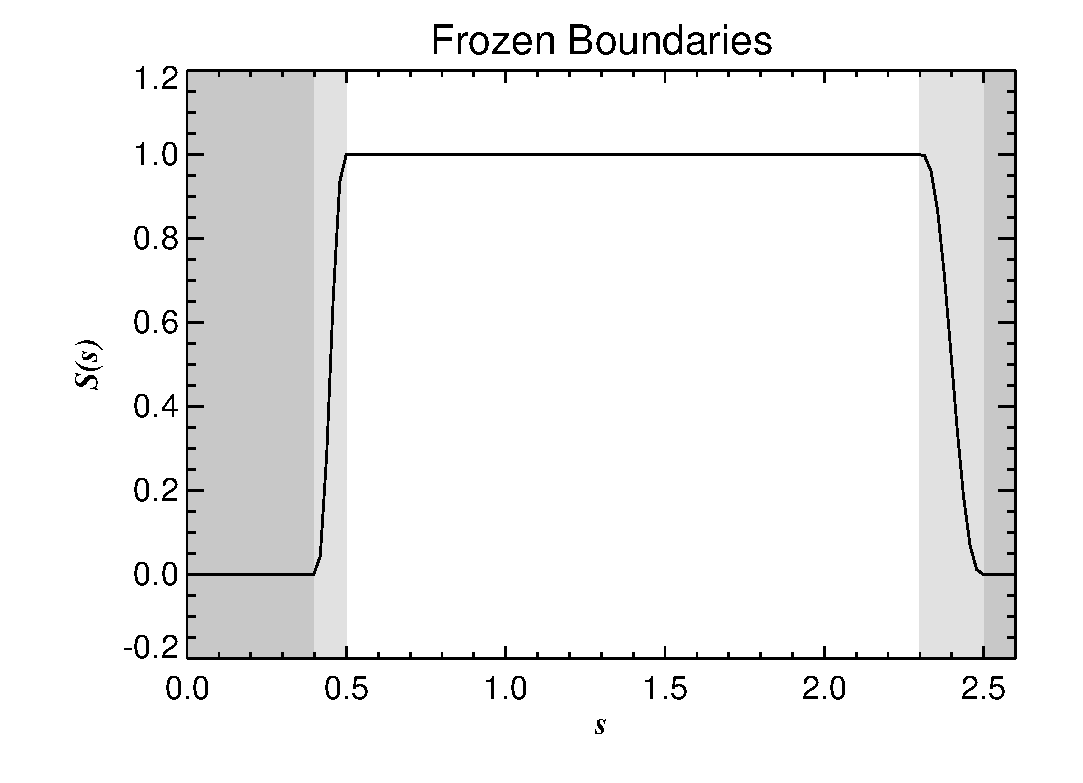
\includegraphics{../figs/freeze.ps}}
\end{center}
\caption[]{Damping and freezing profile to be applied to the derivatives of the variables.}
\end{figure}

Combined, these two functions result in the freezing profile shown in Fig.~\ref{border}. That function multiplies the derivatives of the variables. We simply have to specify that we  want both internal and external freezing for density and velocities by setting 
lfreeze\_uint=T,lfreeze\_uext=T and lfreeze\_lnrhoint=T lfreeze\_lnrhoext=T

Now, the last thing needed is dissipation. For density, we can use upwinding (lupw\_rho=T)

For velocity, a simple viscosity with constant $\nu$ as in Eq.~\ref{navier-stokes} will work well. For the choice of sound speed and length, $10^{-5}$ should do. The {\tt run.in} file should then be

{\tt 
\begin{tabbing}
kkkkkkkkkkkkkkkkkkkkkkkk\=kkkkkkkkkkk\=\kill
! \>                          -*-f90-*-\>     (for Emacs)\\
!  Run parameters!\\
!\\
kkk\=\kill 
\&run\_pars\\
  \>cvsid=`\$Id: hello_disk.tex,v 1.1 2007-09-30 17:31:30 wlyra Exp $',\\
  \>ip=14,\\
  \>nt=50, it1=5, isave=100, itorder=3, ialive=1\\
  \>cdt=0.4,\\ 
  \>cdtv=0.4, \\
  \>dtmin=1e-6,\\
  \>dsnap=6.2831   !VARN for every complete orbit at s0\\
  \>dvid=1.        !video slices more often\\
!\\
  \>wfreeze\_int = 0.05\\
  \>wfreeze\_ext = 0.1\\
  \>fshift\_int=1\\
  \>fshift\_ext=-1\\
!\\
/\\
\&eos\_run\_pars\\
/\\
\&hydro\_run\_pars\\
  \>lfreeze\_uint=T,lfreeze\_uext=T\\
/\\
\&density\_run\_pars\\
  \>lupw\_rho=T\\
  \>lfreeze\_lnrhoint=T\\
  \>lfreeze\_lnrhoext=T\\
/\\
\&grav\_run\_pars\\
/\\
\&viscosity\_run\_pars\\
  \>ivisc='nu-const'\\
  \>nu=1e-5\\
/
\end{tabbing}
}

Now run and relax!

%In 2 dimensions or in the cylindrical gravity approximation, this is all that we need. However, when taking proper care of the vertical direction, density stratification is needed to produce the pressure gradient that counterbalances gravity and ensures vertical hydrostatic equilibrium. 

%\[
%   \ln\rho = \ln\rho(s,\phi) - \frac{z^2}{2H^2} 
%\]where $H$=$c_s/\Omega$ is the pressure scale height. Another way of writing that is via the potential. From the vertical momentum equation, 
%
%\[
%  \ddot{z}=0=-\rho^{-1}\grad{p} - \grad{\Phi}
%\]
%
%As the sound speed does not depend on z, 
%
%\[
%  \pderiv{\ln\rho}{z}=-\frac{1}{c_s^2}\pderiv{\Phi}{z}
%\]


\end{document}
